\documentclass[11pt]{article}
\usepackage[pdftex]{graphicx}
\usepackage{siunitx}
\usepackage{amsmath}
\usepackage{fixmath}
\usepackage[czech]{babel}
\usepackage[utf8]{inputenc}
\usepackage[T1]{fontenc}
\graphicspath{ {./Obrazky/} }
\sisetup{detect-weight=true, detect-family=true}
\begin{document}

\begin{titlepage}
\center

\textbf{\Huge{Elektronika pro informační technologie}}
\\[4.0cm]

\textsc{\Huge Semestrální projekt}
\\[1.0cm]
\Large{Ladislav Ondris (xondri07)}
\\[0.7cm]
\Large{20. 12. 2018}


\end{titlepage}

\newpage
\section{Úloha 1 - varianta C}
Stanovte napětí \(U_{R3}\) a proud \(I_{R3}\). Použijte metodu postupného zjednodušování
obvodu.
\\
\\
\(U_1 = \SI{100}{\volt}\),
\(U_2 = \SI{80}{\volt}\),
\(R_1 = \SI{450}{\ohm}\),
\(R_2 = \SI{810}{\ohm}\),
\(R_3 = \SI{190}{\ohm}\),
\(R_4 = \SI{220}{\ohm}\),
\(R_5 = \SI{220}{\ohm}\),
\(R_6 = \SI{720}{\ohm}\),
\(R_7 = \SI{260}{\ohm}\),
\(R_8 = \SI{180}{\ohm}\)

\begin{center}
	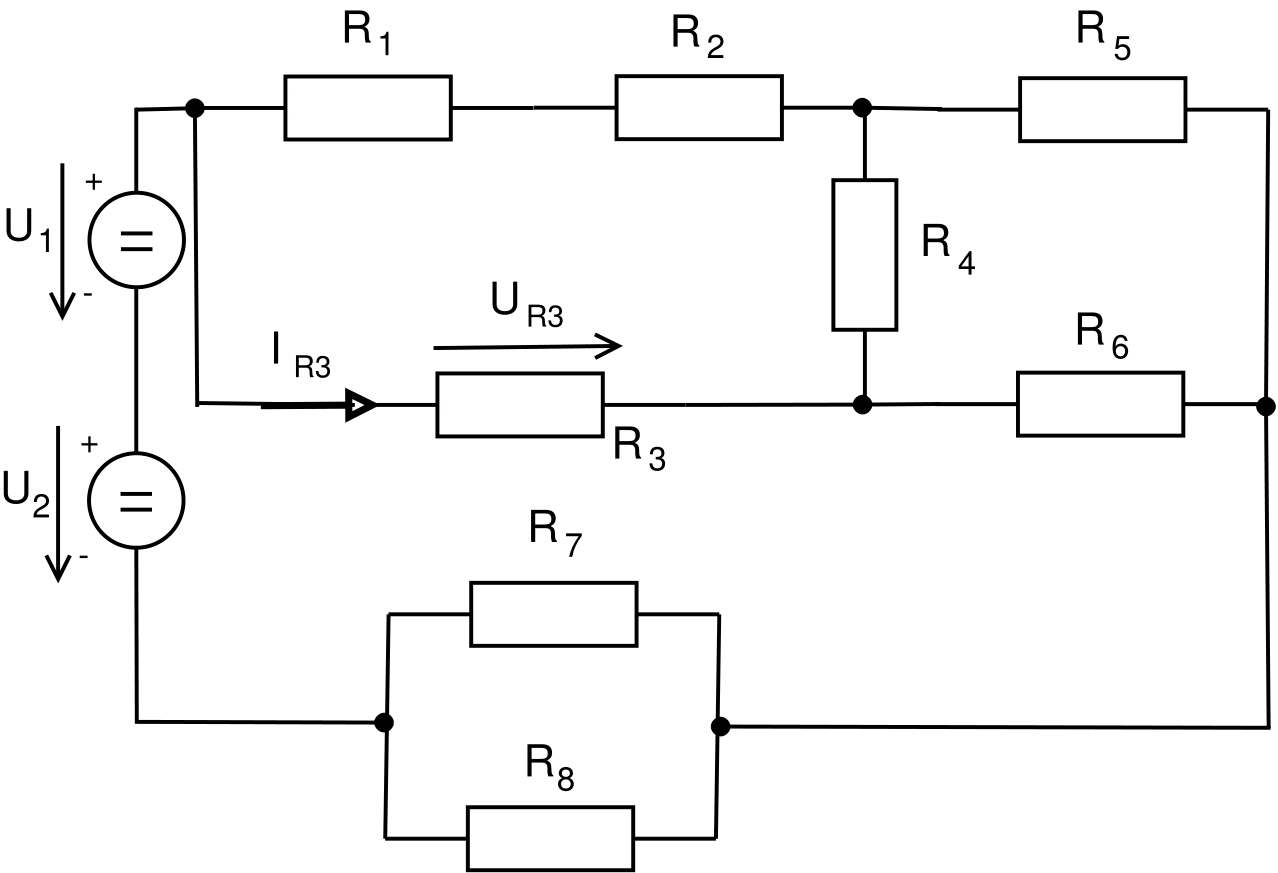
\includegraphics[width=6cm]{Pr1_2018.png} 
\end{center}

Nejprve obvod zjednodušíme do následujícího tvaru.

\begin{center}
	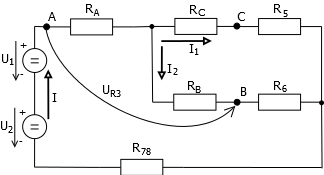
\includegraphics[width=6cm]{Pr1_2018_2.png} 
\end{center}

\(R_1\) a \(R_2 \) jsou sériově.
\[R_{12} = R_1 + R_2 = 450 + 810 = \SI{1260}{\ohm}\]

Nyní můžeme převést rezistory \(R_{12}\), \(R_3\) a \(R_4\) z trojúhelníku na hvězdu.
\[R_A = \frac{R_{12}*R_3}{R_{12} + R_3 + R_4} = \frac{1260 * 190}{1670} = \SI{143.3533}{\ohm} \]
\[R_B = \frac{R_3*R_4}{R_{12} + R_3 + R_4} = \frac{190 * 220}{1670} = \SI{25.0299}{\ohm} \]
\[R_C = \frac{R_{12}*R_4}{R_{12} + R_3 + R_4} = \frac{1260 * 220}{1670} = \SI{165.9880}{\ohm} \]

Rezistory \(R_7\) a \(R_8 \) jsou paralelně.
\[R_{78} = \frac{R_7*R_8}{R_7 + R_8} = \frac{260 * 180}{260 + 180} = \SI{106.3636}{\ohm} \]

Obvod dále zjednodušíme.

\begin{center}
	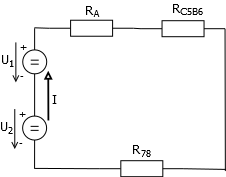
\includegraphics[width=6cm]{Pr1_2018_4.png} 
\end{center}

\(R_C\) a \(R_5\) jsou zapojeny sériově, stejně tak \(R_B\) s \(R_6\).
\[R_{C5} = R_C + R_5 = \SI{385.9880}{\ohm} \]
\[R_{B6} = R_B + R_6 = \SI{745.0299}{\ohm} \]
\(R_{C5}\) a \(R_{B6}\) jsou paralelně.
\[R_{C5B6} = \frac{R_{C5} * R_{B6}}{R_{C5} + R_{B6}} = \SI{254.2600}{\ohm} \]

Nyní máme obvod, kde jsou tři odpory, všechny sériově. Můžeme je tedy zjednodušit na jediný odpor v obvodu.

\begin{center}
	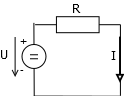
\includegraphics[width=3cm]{Pr1_2018_3.png} 
\end{center}

\[R = R_A + R_{C5B6} + R_{78} = 143.3533 + 254.2600 + 106.3636 = \SI{506.9769}{\ohm} \]

Zdroje napětí můžeme sečíst, neboť jsou zapojeny sériově.
\[U = U_1 + U_2 = 100 + 80 = \SI{180}{\volt} \]

Ohmovým zákonem můžeme spočítat proud.
\[I = \frac{U}{R} = \frac{180}{506.9769} = \SI{0.357159}{\ampere} \]

Zpětně vyjádříme a vypočítáme proudy \(I_1\) a \(I_2\) poměrem:
\[\frac{I_1}{I_2} = \frac{R_{B6}}{R_{C5}} = \frac{745.0299}{385.9880}\]
\[I_1 = I * \frac{R_{B6}}{R_{B6} + R_{C5}} = 0.357159 * \frac{745.0299}{1131.0179} = \SI{0.2352696}{\ampere} \]
\[I_2 = I * \frac{R_{C5}}{R_{B6} + R_{C5}} = 0.357159 * \frac{385.9880}{1131.0179} = \SI{0.1218894}{\ampere} \]

A konečně, můžeme vypočítat \(U_{R3}\) a \(I_{R3}\). Tady nám pomůže II. Kirchhoffův zákon.
\[I R_A + I_2 R_B - U_{R3} = 0 \]
\[U_{R3} = I R_A + I_2 R_B = \textbf{\SI{54.2508}{\volt}} \]
\[I_{R3} = \frac{U_{R3}}{R_3} = \frac{54.2508}{190} = \SI{0.2855305}{\ampere} = \textbf{\SI{285.5305}{\milli\ampere}} \]

\newpage

\section{Úloha 2 - varianta D}
Stanovte napětí \(U_{R1}\) a proud \(I_{R1}\). Použijte metodu Théveninovy věty.
\\
\\
\(U = \SI{150}{\volt}\),
\(R_1 = \SI{200}{\ohm}\),
\(R_2 = \SI{200}{\ohm}\),
\(R_3 = \SI{660}{\ohm}\),
\(R_4 = \SI{200}{\ohm}\),
\(R_5 = \SI{550}{\ohm}\)

\begin{center}
	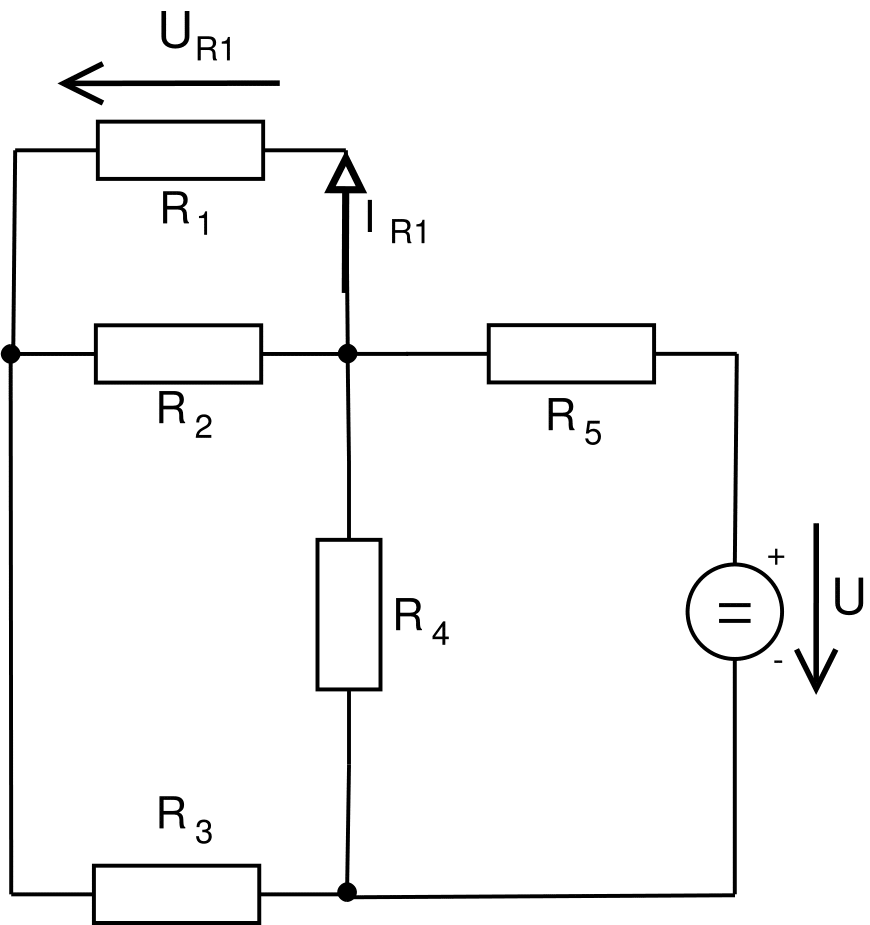
\includegraphics[width=6cm]{Pr2_2018.png} 
\end{center}

Podle Thévinovy věty převedeme obvod na obvod náhradní, který bude vypadat následovně.

\begin{center}
	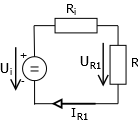
\includegraphics[width=4cm]{Pr2_2018_2.png} 
\end{center}

Odpor \(R_i\) určíme jako odpor mezi svorkami A, B naprázdno.

\begin{center}
	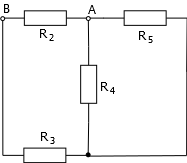
\includegraphics[width=6cm]{Pr2_2018_3.png} 
\end{center}

\[R_{45} = \frac{R_4 * R_5}{R_4 + R_5} = \frac{200 * 550}{750} = \SI{146.6667}{\ohm}\]
\[R_{345} = R_{45} + R_3 = 146.6667 + 660 = \SI{806.6667}{\ohm} \]
\[R_i = \frac{R_2 * R_{345}}{R_2 + R_{345}} = \frac{200 * 806.6667}{1006.6667} = \SI{160.2649}{\ohm} \]

Dále určíme napětí \(U_i\) naprázdno mezi svorkami A, B.

\begin{center}
	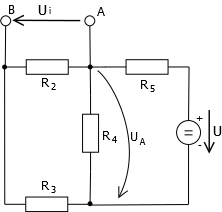
\includegraphics[width=6cm]{Pr2_2018_4.png} 
\end{center}

Odpory \(R_2\), \(R_3\) a \(R_4\) zjednodušíme v jeden odpor \(R_{234}\). 
\[R_{234} = \frac{(R_2 + R_3) * R_4}{R_2 + R_3 + R_4} = \frac{(200 + 660) * 200}{1060} = \SI{162.2642}{\ohm} \]
Poměrem napětí mezi odporem \(R_{234}\) a \(R_5\) zjistíme:
\[U_A = U * \frac{R_{234}}{R_{234} + R_5} = 150 * \frac{162.2642}{162.2642 + 550} = \SI{34.1722}{\volt} \]
\[U_i = U_A * \frac{R_2}{R_2 + R_3} = 34.1722 * \frac{200}{200 + 660} = \SI{7.9470}{\volt} \]



Nyní můžeme z náhradního obvodu spočítat \(I_{R1}\) a \(U_{R1}\).

\begin{center}
	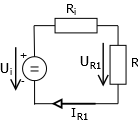
\includegraphics[width=4cm]{Pr2_2018_2.png} 
\end{center}

\[I_{R1}*R_i + I_{R1} * R_1 - U_i = 0 \]
\[I_{R1} = \frac{U_i}{R_i + R_1} = \frac{7.9470}{160.2649 + 200} = \SI{0.0220588}{\ampere} = \textbf{\SI{22.0588}{\milli\ampere}} \]

\[U_{R1} = I_{R1} * R_1 = 0.0220588 * 200 = \textbf{\SI{4.4118}{\volt}} \]
\newpage

\section{Úloha 3 - varianta G}
Stanovte napětí \(U_{R3}\) a proud \(I_{R3}\). Použijte metodu uzlových napětí (\(U_A\), \(U_B\), \(U_C\)).
\\
\\
\(U = \SI{160}{\volt}\),
\(I_1 = \SI{0.65}{\ampere}\),
\(I_2 = \SI{0.45}{\ampere}\),
\(R_1 = \SI{46}{\ohm}\),
\(R_2 = \SI{41}{\ohm}\),
\(R_3 = \SI{53}{\ohm}\),
\(R_4 = \SI{33}{\ohm}\),
\(R_5 = \SI{29}{\ohm}\)

\begin{center}
	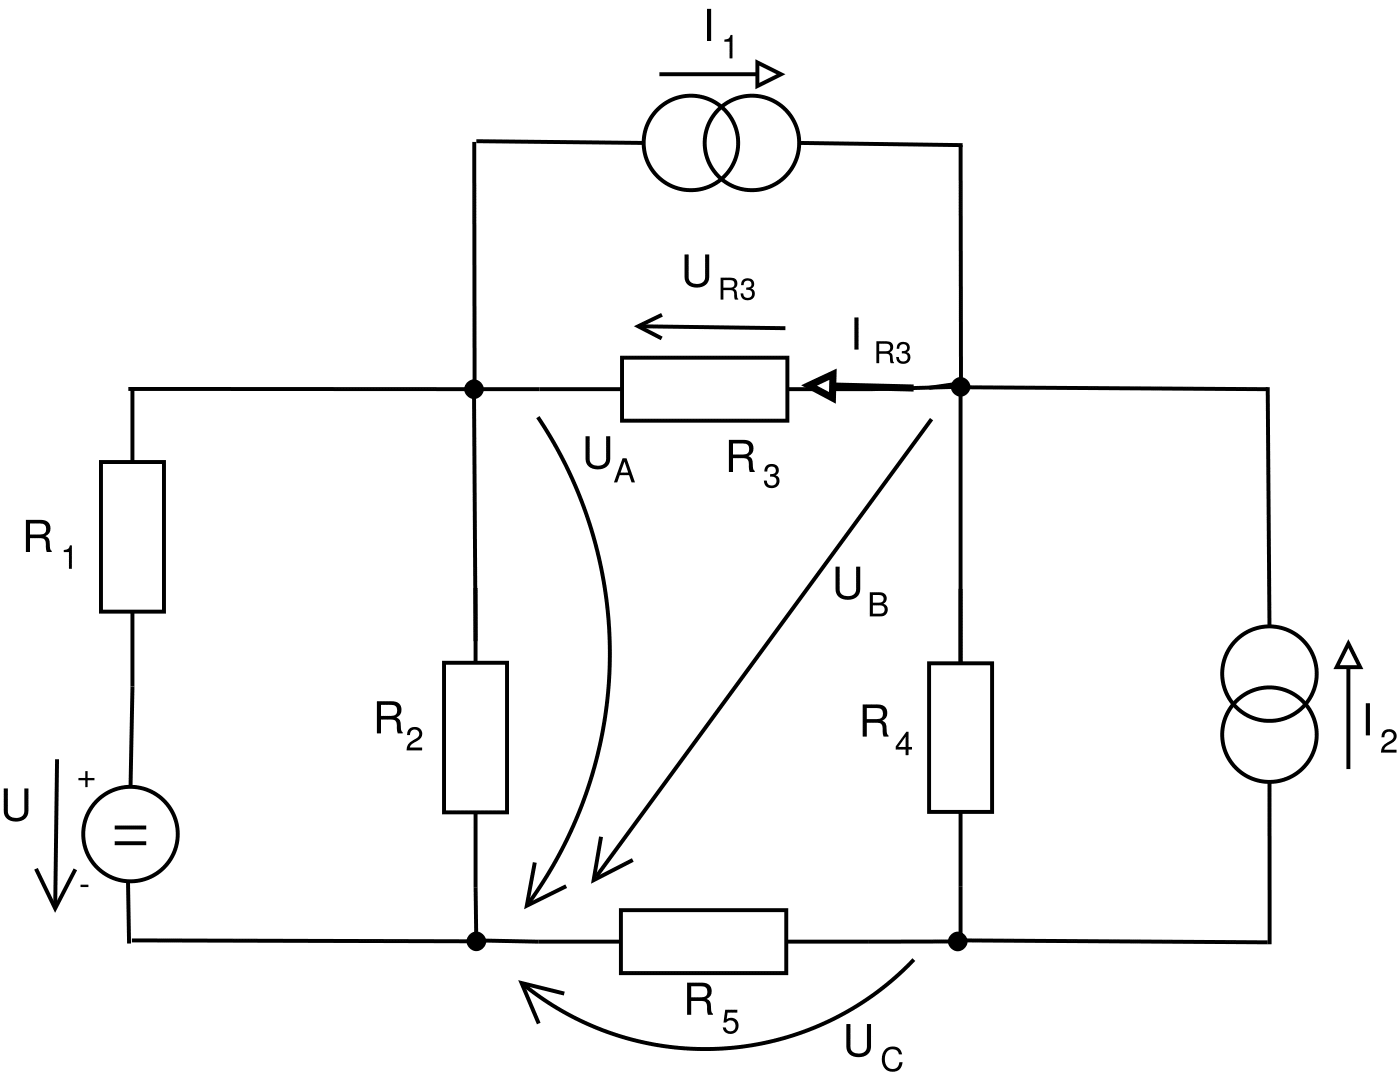
\includegraphics[width=8cm]{Pr3_2018.png} 
\end{center}

Nejprve doplníme nákres o uzlové proudy. 

\begin{center}
	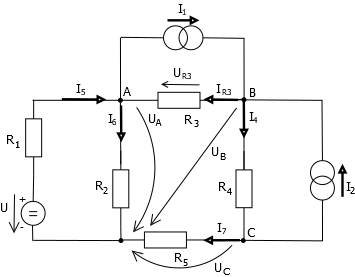
\includegraphics[width=8cm]{Pr3_2018_2.png} 
\end{center}

Napíšeme rovnice pro uzly A, B a C podle I. KZ.

\[A: I_5  + I_{R3} - I_1 - I_6 = 0\]
\[B: I_2  + I_1 - I_{R3} - I_4 = 0\]
\[C: I_4  - I_2 - I_7 = 0\]

Proudy ve větvích uzlu vyjádříme pomocí uzlových napětí a odporů. 

\[I_4 * R_4 + U_C - U_B = 0 \implies I_4 = \frac{U_B - U_C}{R_4}\]
\[I_5 * R_1 + U_A - U = 0 \implies I_5 = \frac{U - U_A}{R_1} \] 
\[I_6 = \frac{U_A}{R_2} \]
\[I_7 = \frac{U_C}{R_5}\]
\[I_{R3} * R_3 + U_A - U_B = 0 \implies I_{R3} = \frac{U_B - U_A}{R_3}\]

Dosadíme do rovnic.

\[\frac{U - U_A}{R_1} + \frac{U_B - U_A}{R_3} - I_1 - \frac{U_A}{R_2} = 0\]
\[I_2 + I_1 - \frac{U_B - U_A}{R_3} - \frac{U_B - U_C}{R_4} = 0\]
\[\frac{U_B - U_C}{R_4} - I_2 - \frac{U_C}{R_5} = 0\]

Dosadíme hodnoty a upravíme.

\[\frac{160 - U_A}{46} + \frac{U_B - U_A}{53} - 0,65 - \frac{U_A}{41} = 0 \quad / \ast 99958\]
\[1,1 - \frac{U_B - U_A}{53} - \frac{U_B - U_C}{33} = 0 \quad / \ast 1749\]
\[\frac{U_B - U_C}{33} - 0,45 - \frac{U_C}{29} = 0 \quad / \ast 957\]


\[347680 - 2173 U_A + 1886 U_B - 1886 U_A - 64972,7 - 2438 U_A = 0 \]
\[1923,9 + 33 U_A - 33 U_B + 53 U_C - 53 U_B = 0\]
\[29 U_B - 29 U_C - 430,65 - 33 U_C = 0\]

\begin{table}[]
	\begin{tabular}{r r r c r}
		-6497 U\textsubscript{A} & +1886 U\textsubscript{B} & & = & -282707,3 \\
		33 U\textsubscript{A}    & - 86 U\textsubscript{B}  & + 53 U\textsubscript{C} & = & -1923,9   \\
		& 29 U\textsubscript{B}    & - 62 U\textsubscript{C} & = & 430,65   
	\end{tabular}
\end{table}


Soustavu lineárních rovnic vyřešíme Cramerovým pravidlem.

\[ |U| =
\begin{vmatrix}
	-6497 & 1886 & 0 \\ 
	33 & -86 & 53 \\ 
	0 & 29 & -62
\end{vmatrix}
= -20797359
\]

\[ |U_A| =
	\frac{
		\begin{vmatrix}
		-282707,3 & 1886 & 0 \\ 
		-1923,9 & -86 & 53 \\ 
		430,65 & 29 & -62
		\end{vmatrix}
	}{|U|}
	= \frac{-1.25479 * 10^9}{-20797359} = \SI{60,3341}{\volt}
\]

\[ |U_B| =
\frac{
	\begin{vmatrix}
	-6497 & -282707,3 & 0 \\ 
	33 & -1923,9 & 53 \\ 
	0 & 430,65 & -62
	\end{vmatrix}
}{|U|}
= \frac{-1.20510 * 10^9}{-20797359} = \SI{57,9449}{\volt}
\]

Nyní se můžeme vrátit k výpočtu \(I_{R3}\). Dříve jsme si ho vyjádřili, nyní můžeme dosadit a spočítat.

\[I_{R3} = \frac{U_B - U_A}{R_3} = \frac{57,9449 - 60,3341}{53} = \SI{-0,0450792}{\ampere} = \textbf{\SI{-45,0792}{\milli\ampere}} \]

Proud vyšel záporný, a tudíž proud teče opačným směrem, než je nakresleno v obrázku.

Podle Ohmova zákona spočítáme napětí \(U_{R3}\).

\[U_{R3} = I_{R3} * R_3 = -0,0450792 * 53 = \textbf{\SI{-2,3892}{\volt}} \]

\newpage
\section{Úloha 4 - varianta C}
Pro napájecí napětí platí: \(u_1 = U_1 \cdot \sin{(2\pi ft)}, u_2 = U_2 \cdot \sin{(2\pi ft)} \). Ve vztahu pro napětí \(u c_2 = U_{C_2} \cdot \sin{(2\pi ft + \varphi c_2)} \) určete \(|U_{C_2}| \) a \(\varphi c_2 \) Použijte metodu smyčkových proudů.
\\
\\
\(U_1 = \SI{35}{\volt}\),
\(U_2 = \SI{45}{\volt}\),
\(R_1 = \SI{10}{\ohm}\),
\(R_2 = \SI{13}{\ohm}\),
\(R_3 = \SI{11}{\ohm}\),
\(L_1 = \SI{220}{\milli\henry}\),
\(L_2 = \SI{70}{\milli\henry}\),
\(C_1 = \SI{230}{\micro\farad}\),
\(C_2 = \SI{85}{\micro\farad}\),
\(f = \SI{75}{\hertz}\)

\begin{center}
	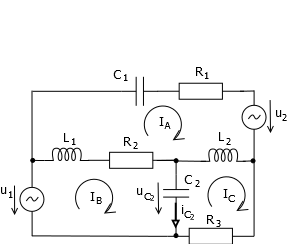
\includegraphics[width=8cm]{Pr4_2018_2.png} 
\end{center}

Víme, že impendance kondenzátoru je \[Z_C = \frac{1}{j{\omega}C} = -\frac{j}{{\omega}C}\]
a impedance cívky je \[Z_L = j{\omega}L \]
\\
Spočítáme si úhlovou frekvenci \[\omega = 2{\pi}f=150f rad/s\]

Sestavíme rovnice pro smyčkové proudy.
\[I_A: Z_{C1}I_A + R_1I_A + U_2 + Z_{L2}I_A - Z_{L2}I_C + R_2I_A - I_BR_2 + Z_{L1}I_A - Z_{L1}I_B = 0\]
\[I_B: -U_1 + Z_{L1}I_B - Z_{L1}I_A + R_2I_B - R_2I_A + Z_{C2}I_B - Z_{C2}I_C = 0\]
\[I_C: R_3I_C + Z_{C2}I_C - Z_{C2}I_B + Z_{L2}I_C - Z_{L2}I_A = 0\]

Upravíme do maticového tvaru a za impedanci dosadíme.

\[
\begin{bmatrix}
-\frac{j}{{\omega}C_1} + R_1 + j{\omega}L_2 + R_2 + j{\omega}L_1 & -R_2 - j{\omega}L_1 & -j{\omega}L_2 \\
-j{\omega}L_1 - R_2 & j{\omega}L_1 + R_2 - \frac{j}{{\omega}C_2} & \frac{j}{{\omega}C_2} \\
-j{\omega}L_2 & \frac{j}{{\omega}C_2} & R_3 - \frac{j}{{\omega}C_2} + j{\omega}L_2
\end{bmatrix}
\begin{bmatrix}
I_A \\
I_B \\
I_C
\end{bmatrix}
=
\begin{bmatrix}
-U_2 \\
U_1 \\
0
\end{bmatrix}
\]

Dosadíme hodnoty a upravíme.

\[
\begin{bmatrix}
23 + 127.4329j & -13 - 33{\pi}j & -\frac{21}{2}{\pi}j \\
-13 - 33{\pi}j & 13 + 78.7071j & 24.9655j \\
-\frac{21}{2}{\pi}j & 24.9655j & 11 + 8.0212j
\end{bmatrix}
\begin{bmatrix}
I_A \\
I_B \\
I_C
\end{bmatrix}
=
\begin{bmatrix}
-45 \\
35 \\
0
\end{bmatrix}
\]

Soustavu lineárních rovnic vyřešíme Cramerovým pravidlem a determinanty matic Sarussovým pravidlem.

\[
	|M| = 
		\begin{vmatrix}
		23 + 127.4329j & -13 - 33{\pi}j & -\frac{21}{2}{\pi}j \\
		-13 - 33{\pi}j & 13 + 78.7071j & 24.9655j \\
		-\frac{21}{2}{\pi}j & 24.9655j & 11 + 8.0212j
		\end{vmatrix}
		= 10210.96939 + 9602.47036j
\]

\[
I_B = 
\frac
{
	\begin{bmatrix}
	23 + 127.4329j & -45 & -\frac{21}{2}{\pi}j \\
	-13 - 33{\pi}j & 35 & 24.9655j \\
	-\frac{21}{2}{\pi}j & 0 & 11 + 8.0212j
	\end{bmatrix}
}
{
	|M|
} 
= \]
\[= \frac{5090.74178 - 491.58550j}{10210.96939 + 9602.47036j} = 0.24055 - 0.27436j
\]

\[
I_C =
\frac
{
	\begin{vmatrix}
	23 + 127.4329j & -13 - 33{\pi}j & -45 \\
	-13 - 33{\pi}j & 13 + 78.7071j & 35 \\
	-\frac{21}{2}{\pi}j & 24.9655j & 0
	\end{vmatrix}
}
{
	|M|
} 
= \]
\[= \frac{-7981.3724 - 9780.68397j}{10210.96939 + 9602.47036j} = -0.89283 - 0.11823j
\]

Vypočítáme proud na kondenzátoru.

\[i_{C2} = I_B - I_C = (0.24055 - 0.27436j) - (-0.89283 - 0.11823j) = 1.13338 - 0.15613j\]

Spočítáme napětí \( U_{C2} \).

\[U_{C2} = i_{C2} * Z_{C2} = i_{C2} * (-\frac{j}{{\omega}C_2}) = (1.13338 - 0.15613j)(-24.96548j) = -3.89786 - 28.29538j\]

Vypočítáme \(|U_{C2}|\) a \({\varphi}_{C2}\). Protože jsme ve 3. kvadrantu, nesmíme zapomenout připočítat 180 stupňů.

\[ |U_{C2}| = \sqrt{Re(U_{C2})^2 + Im(U_{C2})^2} = \sqrt{(-3.89786)^2 + (-28.29538)^2} = \textbf{\SI{28.56259515}{\volt}}\] 

\[ {\varphi}_{C2} = arctan\frac{Im(U_{C2})}{Re(U_{C2}} = 180 + arctan\frac{-28.29538}{-3.89786} = 180 + 82.15652519 = \textbf{\ang{262.15652519}}\]



\newpage
\section{Úloha 5 - varianta D}
Sestavte diferenciální rovnici popisující chování obvodu na obrázku, dále ji upravte dosazením hodnot parametrů. Vypočítejte analytické řešení \(u_C = f(t) \). Proveďte kontrolu výpočtu dosazením do sestavené diferenciální rovnice.
\\
\\
\(C = \SI{5}{\farad}\),
\(R = \SI{25}{\ohm}\),
\(u_C(0) = \SI{6}{\volt} \)

\begin{center}
	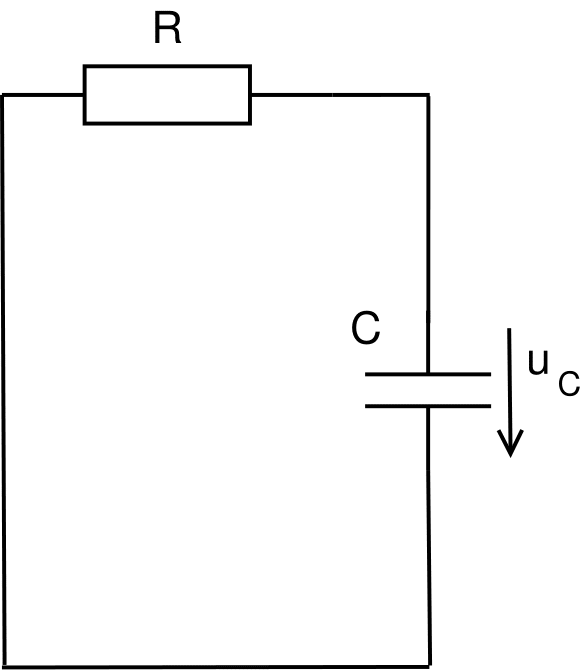
\includegraphics[width=5cm]{Pr5_2018.png} 
\end{center}

Než diferenciální rovnici budeme řešit, nejprve ji musíme sestavit. 

Víme následující:
\begin{enumerate}
	\item \( i = \frac{u_R}{R} \)
	\item \( u_R + u_C = 0 \)
	\item \( u_C' = \frac{1}{C}i_C = \frac{i}{C} \)
\end{enumerate}

Počáteční podmínka: \( u_c(0) = u_{cp} \)
\\

Budeme dosazovat tyto rovnice vzájemně do sebe takovým způsobem, abychom dostali jedinou rovnici, v které bude \(u_C\) a \(u_C'\).

a) dosadíme 1. rovnici do 3.
\[ u_C' = \frac{i}{C} = \frac{u_R}{RC} \]

b) vyjádříme \( u_R \) z 2. rovnice a dosadíme do a)
\[ u_R = -u_C \]
\[ u_C' = \frac{u_R}{RC} = -\frac{u_C}{RC} \]
\[ u_C' + \frac{u_C}{RC} = 0\] 
Získali jsme homogenní diferenciální rovnice 1. řádu.
\\
Nyní diferenciální rovnici vyřešíme.

$$ \si{\micro}(t) = e^{\int\frac{1}{RC} dt} = e^{\frac{t}{RC}} $$
Vynásobíme celou rovnici $ e^{\frac{1}{RC}t} $
$$ e^{\frac{t}{RC}} \cdot u_C' + \frac{1}{RC} \cdot e^{\frac{t}{RC}} \cdot u_C = 0  $$

Podle product rule z pravidel pro derivace můžeme rovnici zapsat ve tvaru

$$ (e^{\frac{t}{RC}} \cdot u_C)' = 0 $$

Když rovnici zintegrujeme, dostaneme:

$$ e^{\frac{t}{RC}} u_C = k $$

\textbf{Obecné řešení} rovnice je:
$$ u_C(t) = k \cdot e^{-\frac{t}{RC}} $$

Dosadíme do počáteční podmínky $ u_C(0) = u_{cp} $
$$ u_{cp} = e^{-\frac{0}{RC}} $$
$$ u_{cp} = k $$

\textbf{Skutečné řešení} je tedy: 
$$ u_C(t) = u_{cp} \cdot e^{-\frac{t}{RC}} $$

Po dosazení konkrétních hodnot dostáváme výsledné řešení:

$$ \mathbold{u_C(t) = 6\cdot e^{-\frac{t}{125}}} $$

Provedeme zkoušku, zda skutečné řešení je opravdu naším řešením. 
Dosadíme do počáteční rovnice $ u_C(t) $ a $ u_C'(t) $.

Dosadíme tedy
$$ u_C(t) = u_{cp} \cdot e^{-\frac{t}{RC}} $$
$$ u_C'(t) = -\frac{u_{cp}}{RC} \cdot e^{-\frac{t}{RC}} $$
do
$$ u_C' = -\frac{u_C}{RC} $$
a dostaneme
$$ -\frac{u_{cp}}{RC} \cdot e^{-\frac{t}{RC}} = -\frac{u_{cp}}{RC} \cdot e^{-\frac{t}{RC}} $$

Řešení je tedy správné.


\newpage
\section{Tabulka s variantami úloh a výsledky}
	
		\begin{tabular}{|l|l|l|}
			\hline
			Úloha & Varianta & Výsledky     \\ \hline
			1     & C        & \(I_{R3} = \SI{285.5305}{\ampere}, U_{R3} = \SI{54.2508}{\volt}\) \\ \hline
			2     & D        & \(I_{R1} = \SI{22.0588}{\milli\ampere}, U_{R1} = \SI{4.4118}{\volt}\) \\ \hline
			3     & G        & \(I_{R3} = \SI{-45.0792}{\milli\ampere}, U_{R3} = \SI{-2.3892}{\volt}\) \\ \hline
			4     & C        & \(|U_{C2}| = \SI{28.5625}{\volt}, {\varphi}_{C2} = \ang{262.1565}\) \\ \hline
			5     & D        & $ u_C(t) = 6\cdot e^{-\frac{t}{125}} $ \\ \hline
		\end{tabular}
	
\end{document}